The previous sections describe about the importance of Read Copy Update (RCU) in parallel programming paradigm and rules one should follow to correctly use the RCU primitives. It also describes about the violation of RCU rules, which can be a potential bug in program, and challenges involved in identifying such bugs. There are existing solution like static analysis~\cite{sparse}, lockdep-RCU~\cite{PaulEMcKenney2010LockdepRCU} etc which is used to identify such bugs but they are imprecise and generate false positive.

Our approach to identify the such RCU bugs involves the technique of Dynamic Binary Instrumentation (DBI). Dynamic Binary Instrumentation (DBI) is an execution control and analysis technique that involves injecting binary code into a running program. The injected code is term “Instrumentation”. There are many DBI infrastructure exist like DynamoRIO~\cite{Bruening04efficient}, DynamoRIO Kernel (DRK)~\cite{Feiner:2012:CKI:2150976.2150992},  Pin~\cite{Bungale:2007:PPF:1254810.1254830}, JIFL~\cite{Olszewski:2007:JIN:1272996.1273000}, KernInst~\cite{Tamches:1999:UDK:1080598.1080605} etc which provides support for fine-grained monitoring and program execution. Our system uses Granary~\cite{GranaryAtOSDI}, a comprehensive kernel module instrumentation framework. The choice of Granary as DBI framework is based on the fact that it provides the support for instrumenting only kernel modules and thus incur no overhead when non-module code executes. Granary allows the interaction between the kernel and module through wrappers having rich information about kernel and its types, thus giving us the complete control on all the data passed over it. It also provide the infrastructure for adding watchpoint for all the memory addresses passed over the wrapper. Our decision to use Granary as the DBI framework is also based on the fact that we used rcu torture test module to evaluate our system which needs the instrumentation of only module code. 


\subsection{Granary}
Granary~\cite{GranaryAtOSDI} is a Dynamic Binary Instrumentation (DBI) framework, developed over DynamoRIO Kernel (DRK) and provides support for fine-grained instrumentation of only kernel modules. Granary gets loaded as the kernel module and interposes during module loading mechanism to generate the module wrapper. It also use the rich kernel type informations to generate a static kernel wrapper. Once the module gets loaded, it runs under the control of Granary and all interactions between the kernel and module happens through one of these wrappers. The presence of these wrappers provides an efficient infrastructure to monitor all the pointers passed from the kernel to the module and add watchpoint on them. The rich kernel type information at the wrapper layer provides support for adding type-based watchpoint on the pointers. However for this project we are using simple watchpoint implementation for tracking the use of RCU primitive and access of RCU protected data. The detail of watchpoint implementation and its usage is provided in next section. 


\subsection{Behavioural Watchpoint}
Watchpoints are an integral feature of program analysis and debugging tools because they correlate watched memory locations with the program points accessing those memory locations. There are two categories of watchpoints: hardware-based and software-based. Hardware-based watchpoints are fast but scarce, which limits their usefulness as a means of perfoming large-scale program analyses \cite{UnlimitedWatchpoints}. Software-based implementations can scale to support millions of watchpoints \cite{Zhao:2008}, but are limited by their view of memory as an opaque sequence of bytes. This view is at odds with program analysis tools, which require contextual information about a program's memory. The watchpoint-based analysis tools are harder to design and implement because they must maintain separate bookkeeping mechanisms to recover contextual information about watched memory. These contextual informations are important when used for analysing the access of RCU protected memory. To achieve our goal, we introduce \emph{behavioural watchpoints}: a new form of software-based watchpoints that simplify the context based program analysis and debugging.  Behavioural watchpoints address the usability concerns of hardware-based watchpoints and overcome the incongruency between how software implements watchpoints and how program analysis tools use watchpoints.

Two characteristics define our behavioural watchpoints:
\begin{enumerate}
	\item[i)] Context-specific information is embedded in each watchpoint. This information is directly available and can be updated when watched address is accessed.
	\item[ii)] The action taken when a watched address is accessed is a component of the context-specific information. This implies that different watchpoints can \emph{behave} differently.
\end{enumerate} 

Implementing software based behavioural watchpoint, without any architectural support, is expensive since it requires to inspect all memory operations and trigger a callback based on the context. A naive approach of implementing watchpoints using dynamic binary instrumentation adds new instructions across every memory references to performs the following task: 
\begin{enumerate}
	\item[i)] Determine the list of addresses which needs to be watched and check if the program is referring to one of the watched addresses.  
	\item[ii)] Check the contextual information and raise a callback when memory operation happens at one of the watched addresses.
	\item[iii)] Incase the address is not one of the watched addresses, continue the normal execution.
\end{enumerate} 
 
The naive system maintains a watchlist lookup table to maintain the list of addresses to be watched and uses an efficient algorithm to look for the addresses.% in the list. One of the drawback of this approach is the runtime overhead, which incurs due to address lookup for every memory addresses.  
To achieve our design goal, we implemented watchpoints by adding an extra level of indirection to memory addresses. An unwatched address is converted into a watched address by changing its high-order bits. These high-order bits indirectly identify context-specific information about the range of memory being watched. This information, called the watchpoint's \emph{descriptor}, contains the originating watched address and a set of functions to invoke when watched memory is dereferenced. Since watchpoint information is embedded in only the high-order bits, a typical offset of a watched address is another watched address that shares the same watchpoint-specific high-order bits. A watchpoint's descriptor is indirectly located by interpreting these high-order bits as an index into a global \emph{watchpoint descriptor table} (\Figref{watchpoint_descriptor_table})

Our approach has the following design implications which is useful for debugging the RCU based applications.

%Any unwatched address can be converted into an watched address. The extra level of indirection added by watching an address allows us to efficiently locate context-specific information about the memory being watched.

%A watchpoint is added to a program by changing the high-order order bits of an address used by the program. 
%Watchpoints work on ranges instead of individual units of memory because a watchpoint is added to a program by changing 

\paragraph{A watched address must be distinguishable from an unwatched address.}All watched addresses are non-canonical addresses that trigger a hardware exception when dereferenced. We take advantage of the x86-64 architecture for implementing watched addresses. In kernel space on x86-64, canonical addresses have their 16 high-order bits set to 1. Watched addresses do not take this form. To prevent hardware exceptions, instrumentation is dynamically added to memory loads and stores. Watched addresses are detected before they are dereferenced and resolved to their unwatched counterparts (by masking the 16 high-order bits to 1). An alternative approach is to dereference a watched address and implement behavioural watchpoints in the trap handler.
	
\paragraph{Multiple watchpoints can watch the same range of memory.}Two copies of an address (e.g.,two pointers to the same object) can be separately watched, so long as the pattern of their high-order bits is different. This is useful for distinguishing between logically different objects that occupy the same memory. This features enables the detection of RCU usage bugs involving violation of Rule 1. %For example, this feature enables efficient detection of use-after-free bugs without preventing deallocated memory from being immediately reallocated for another use. This efficiency comes from our ability to have one watchpoint for the freed memory, and another watchpoint for newly allocated memory occupying the same space.
	
\paragraph{Watchpoints are viral.}If an address $A$ is watched, then every address derived from $A$ (e.g. through copying or offsetting) is also watched. This is useful for memory and taint analysis tools: a watchpoint that is added early on in the lifetime of an address (e.g., immediately before the address of some newly allocated memory is returned from an allocator) can persist and propagate until no more derived addresses exist.

\begin{figure}[t]
\begin{center}
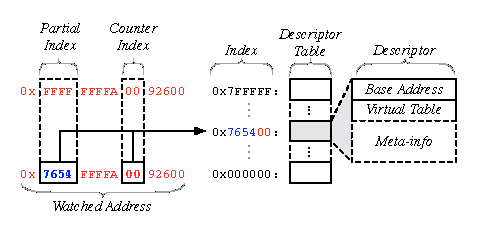
\epsfig{file=watchpoints.eps}
\end{center}
\caption{\label{fig:watchpoint_descriptor_table}A watched address (bottom left) and its corresponding unwatched address (top left) are compared. The process of resolving the watchpoint descriptor for the watched address is shown.}
\end{figure}

\paragraph{Millions of watchpoints are supported.}Our design as described uses 15 of the 16 high-order bits (called the \emph{partial index}) of a watched address for identifying a watchpoint's descriptor. 15 bits only allows 32K watchpoints. To increase the number of watchpoints, we use an additional 8 bits (bits 20-27, called the \emph{counter index}) in the address to index into the watchpoint descriptor table (\Figref{watchpoint_descriptor_table}). This counter index extends the number of possible watchpoints to 8M and is left unchanged when converting an unwatched address into a watched address. The key advantage of our watchpoint scheme is the ability to directly map watched addresses to unwatched addresses using a simple bitmask. The main drawback of the scheme is that an offset of a watched address can cause the low-order bits to overflow into the counter index. We are exploring several solutions to this problem.

%This approach has some drawbacks when an offset of a watched address causes the low-order bits to overflow into the counter index; however, we have several solutions to this problem. 

\paragraph{Watchpoint descriptors can be arbitrarily customized.}This aspect of watchpoints is possible because our design separates the allocation/management of descriptors and the addresses that they watch. Arbitrary extension of descriptors supports our goal of overcoming the incongruency between the needs of debugging an analysis tools (contextual information about watched memory), and how existing software implements watchpoints (watched memory is opaque).

%\subsection{Extensions}
%Our design includes the following extensions to watchpoints, which expand on the behavioural aspect of our watchpoint implementation.
%principally enable the \emph{behavioural} aspect of our software-based watchpoint .
%Our goal of using watchpoints to watch the memory of objects required the following 

%\paragraph{Watchpoints are type-specific.} When a watchpoint is added to an address, the \emph{type} of the address determines what meta-information is included in the descriptor, as well as what functions to invoke when memory watched by the watchpoint is accessed. Two powerful applications of this extension are discussed in \Secref{type_overflow} and \Secref{access_policies}.

%\paragraph{Triggered watchpoint functions are polymorphic.} The function invoked when watched memory is accessed is decided using a descriptor-specific virtual table (vtable). Each vtable provides eight functions: four read and four write functions. Each function is specific to a memory operand size (1, 2, 4, or 8 bytes). A watchpoint descriptor is initialised with either a generic or a type-specific vtable. Type-specific vtables are specific to the \emph{type} of the watched address. Vtables earn behavioural watchpoints their name because they allow watchpoints to behave differently when watched memory is accessed.

%When invoked, a vtable function operates on the watched address and its descriptor. Behavioural watchpoints earn their name from their ability to behave differently based on the meta-information stored in the descriptor and the (type-specific) vtable function invoked.

%\paragraph{Watchpoints remember their originating address.} The address to which a watchpoint is first added is called its \emph{base address}, and is stored in the watchpoint descriptor. We designed watchpoints to remember their base address because it helps to ``anchor" contextual information. When a watchpoint is added, \emph{something} is known about the watched address. Later in a program's execution, an offset of the watched address might be dereferenced. Little can be said about the dereferenced address in relation to the watchpoint's originating address without knowing the originating address.

%Program debugging is a inevitable task in software development process. An efficient debugger can make programmers more productive by allowing them to monitor the execution, inspect the state of the process and monitor memory read and write to inspect the data flow and corruption~\cite{Zhao:2008}. This increases the requirement of an efficient debugging tool supporting an useful feature called \emph{Watchpoints}. The need of such debugging tool increases, as the complexity of the program grows such as parallel system. \emph{Watchpoint} allow a developer to demarcate a memory region and take control whenever that gets accessed. It then ensures the safe access of the memory addresses by checking certain policy. It is similar to the instruction breakpoints which allows the developer to pause execution at specific instructions.

%Implementing software watchpoint, without any architectural support, is expensive since it requires to inspect all memory operations and trigger a callback on the watched addresses. Our system leverages the advances in binary instrumentation and code manipulation technique to provide the efficient feature to add watchpoint at memory addresses. Our system uses this feature to check the correct usage of RCU synchronization primitive and access of RCU protected data, thus identifying the violation of rules and possible buggy usage of RCU.

%The naive approach of implementing watchpoint using dynamic binary instrumentation adds new instructions across every memory references to performs the following task: 
%\begin{itemize}
%	\item Determine the list of addresses which needs to be watched and check if the program is referring to one of the watched addresses.  
%	\item Raise a callback when memory operation happens at one of the watched addresses.
%	\item Incase the address is not one of the watched addresses, continue the normal execution.
%\end{itemize}  
%The naive system also maintains a watchlist lookup table to maintain the list of addresses to be watched. It uses an efficient algorithm to look for the addresses in the list before making a callback on watched addresses. One of the drawback of this approach is the runtime overhead, which incurs due to address lookup for every memory addresses. This makes the implementation of watchpoint costly. 
%\begin{figure}
%\centering
% 	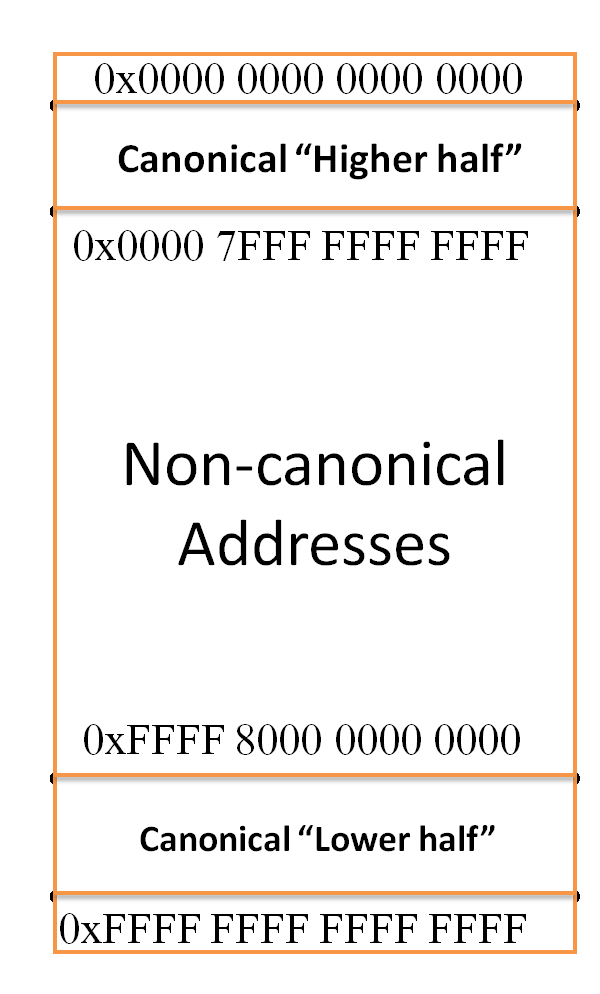
\includegraphics[width=0.2\textwidth]{Picture3-png}
%\caption{64-bit address-space layout (48bit implementation)}\label{fig:addrspace}
%\end{figure}

%Our system refines the cost of adding watchpoint by substantially reducing the cost of lookup and providing options for faster lookup of meta information in shadow memory. The detail about shadow memory and meta information is provided in next section. We took the advantage of 48 bit implementation in 64-bit architecture and used non-canonical addresses to implement our watchpoint mechanism. The use of non-canonical address provides us the following advantages :
%\begin{itemize}
%	\item It decreases the cost of lookup as the non-canonical addresses can be easily recognised by masking lower 48 bits of the addresses.
%	\item It also provides one to one mapping between the actual address and watched address thus proving virtually no cost for fixing the address.
%	\item The unused 15 bits in non-canonical address is used to encode information about the shadow memory storing meta-informations.
%	\item The pointer aliasing the watched address also gets watched, thus there is no need to implement a pointer tracking mechanism.
%\end{itemize}   

%Figure~\ref{fig:addrspace} shows the address-space layout in 64 bit architecture with 48 bit implementations. 
%The highest 1 bit (sign bit) is used for adding watchpoint and differentiate between original and watched addresses. The next 15 bit of address is used to for storing shadow memory index storing meta-information. Our method of storing shadow memory index puts a limit on our system in terms of number of active watchpoint we can add at a time, but we consider this is enough for our project to track the rcu protected data. Figure~\ref{fig:watchpoint} shows the detail, how the watched address gets created.

%\begin{figure}[h]
%\centering
% 	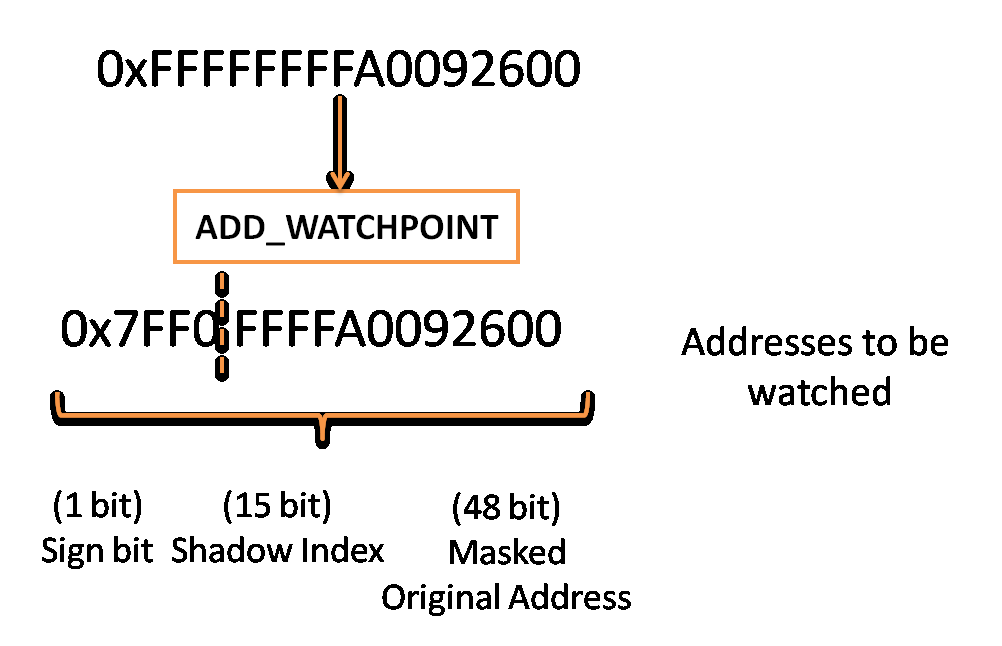
\includegraphics[width=0.4\textwidth]{Picture6-png}
%\caption{Generated Watchpoint Address}\label{fig:watchpoint}
%\end{figure} 

\subsection {Instrumentation and Optimizations}
Watchpoints essentially requires monitoring of every memory read (load) and write (store) operations. A basic monitoring approach using dynamic binary instrumentation adds new instructions before every memory references looking for one of the watched address. %In our system these watched addresses includes non-canonical addresses generated out of original address and the index of shadow memory storing required meta-information. The detail of watchpoint implementation is provided in previous subsection. 
The instrumentation required for implementing watchpoint perform the following operation before every memory references: 

\begin{enumerate}
	\item[i)] Save and restore the registers that are used or side-effected during watchpoint lookup( stack is used to spill these registers ).
	\item[ii)] Calculate the reference address and check if this is one of the non-canonical addresses. Inject a callback function, if the address is one of the non-canonical one. 
	\item[iii)] Emulate the actual instruction with corrected address and continue the execution after restoring registers.
	\item[iv)] Follow the normal course of execution if the address is not one of the watched addresses.
\end{enumerate}

Figure~\ref{fig:mem-write} shows the example of basic instrumentation required for every memory operations. The naive instrumentation suffers from a significant runtime overhead. We implemented and applied some of the optimization to systematically improve the runtime performance. %We used the following optimizations: 
\begin{itemize}
	\item \emph{Dead Registers Analysis:} Every instrumentation system needs scratch registers for creating and injecting new instructions. These registers can be obtained by spilling them to stack or memory locations. %Our naive instrumentation uses stack to spill these registers. 
The frequent spilling of these registers on stack or memory location increases the cost of instrumentation significantly~\cite{Probst02registerliveness, Muth98registerliveness}. Our system performs the register liveness analysis on each basic block to identify registers that can be safely used without requiring it to spill on the stack. For register liveness analysis, our system starts instrumenting from the end of the basicblock moving upward and collecting all the source and destination registers making all the non source and non base-displacement registers (whole destination registers) as dead.  
	\item \emph{Flag Liveness Analysis:} %Instrumentation can change  , we also need to save and restore the flags as the instrumented code modifies the flag. 
One important optimization in instrumentation is Flag Liveness analysis. We save and restore the flag only when it is alive. To identify the dead flag as we move upward instrumenting basic block, we find if any of the instruction modify the flags we consider the instruction previous to that as having dead flag. 
	\item \emph{Merge Checks:} We also exploited the locality of memory references and two instructions in the same basic block accessing the same object or different member of same object (like \emph{0x0(\%rax) and 0x8(\%rax)}) doesn’t require the instrumentation of all references and thus the checks for all of them is merged together.
    \item \emph{Eliminate Stack Operations:} For x86 architecture, any operation on the stack or involving stack pointer is also considered as memory operation. Our system identify all these instructions involving operations on the stack and they are not required to be instrumented since we are not tracking or adding watchpoint on them.
\end{itemize}

\begin{figure}[ht!]
%
\framebox{\begin{minipage}[t]{1.02\columnwidth}%
\vspace{-1em}
\begin{codebox}
\Procname{$\proc{Native-Memory-Operation}$}
\li  mov $\id{\%rsi   -> [\%rax, \%rbx]}$ 
\end{codebox}%

\begin{codebox}
\Procname{$\proc{Instrumented-Memory-Operation}$}
\li  	push 	$\id{\%rcx}$
\li  	push 	$\id{\%rdi}$
\li 	lea 	$\id{[\%rax, \%rbx] 	-> 	\%rdi}$
\li 	pushf
\li 	movabs 	$\id{0xffff000000000000		->	\%rcx}$
\li	or 	$\id{\%rcx 	->	\%rdi}$
\li	cmp 	$\id{\%rdi 	->	\%rdi}$
\li	je     	$\id{addr\_not\_watchpoint}$
\li	popf
\li 	$\proc{insert\_clean\_call}(\id{watch\_write}, \id{\%rdi}, \id{1})$
\li	mov    	$\id{\%rsi	->	[\%rdi]}$
\li	pop	$\id{\%rdi}$
\li	pop 	$\id{\%rcx}$
\li	jmp 	$\id{done\_instrumenting}$
\li	LABEL:  $\id{addr\_not\_watchpoint}$
\li	popf
\li	pop	$\id{\%rdi}$
\li	pop 	$\id{\%rcx}$
\li  	mov 	$\id{\%rsi   	-> 	[\%rax, \%rbx]}$ 
\li	LABEL:  $\id{done\_instrumenting}$
\li  	nop	
\end{codebox}%
\end{minipage}}

\caption{Native and Instrumented memory write Operation\label{fig:mem-write}}
\vspace{-1em}
\end{figure}

%The optimization discussed above improved the performance of watchpoint significantly, but 
Apart from the above, there is a scope of further optimization and one of them is using policy based instrumentation. Policy based instrumentation will only instruments the memory references when execution enters in RCU critical section and any access outside critical section is incorrect and will get trapped by the general protection fault. However this is a big optimization but we have not implemented this since it requires a mechanism of tagging basic block so that two version of basicblock exist in the codecache for same native code, which is currently not supported with Granary.


\begin{figure*}[htb]
%\centering
\begin{lstlisting}
/* Thread-specific watchpoint meta information. */
struct alias_meta_thread {
    alias_meta_thread *next;

    /* writer thread_id + 1 iff this RCU-protected structure is being
     * written to; otherwise 0. An RCU-protected structure is writable from
     * the time of allocation up until it is published using rcu_assign_pointer.
     */
    uint64_t writer_thread_id;

    /* The "generation" number of the thread */
    uint64_t gen_nums[NUM_THREADS];
};

union alias_meta {
        /* if this watchpoint aliases another watchpoint */
        alias_meta *source;
        /* thread info about a source watchpoint */
        alias_meta_thread *thread_info;
}; 
\end{lstlisting}
\caption{Meta-Information: data structure used for meta-info}\label{fig:metainfo}
\end{figure*}

\subsection{Shadow memory and meta information}
This section describes about the type of contextual-information needed and how it is important for debugging RCU based applications. Implementing shadow memory~\cite{Memcheck} is important for behavioural watchpoint since it stores the watchpoint contextual information. These contextual informations is used for tracking RCU primitives and verifying memory access policies for RCU protected data. We store two forms of contextual information in the form of meta-data : \emph{per-thread metadata} and \emph{per-object metadata}.
%tracking the usage of RCU synchronization primitive. The two types of meta-information used are follows: 
\paragraph{Per-thread metadata} It includes thread \emph{generation number} stored at the thread local slot created at the bottom of the stack and used for keeping track of the rcu read critical section.% and used to validate the correct usage of RCU protected data.
\paragraph{Per-object metadata} It includes watchpoint \emph{generation number} and writer\_thread\_id. Watchpoint \emph{generation number} along with thread \emph{generation number} is used to verify the memory access policy. It also stores the information if the watchpoint pointer is source or one of the alias of source pointer generated by \texttt{rcu\_dereference}. %The structure of the per pointer meta-information is shown in the figure~\ref{fig:metainfo}. 

The per-object metadata stored in watchpoint descriptor table includes the thread specific informations(watchpoint generation number) for all the running threads and writer thread ID as shown in figure~\ref{fig:metainfo}. In our implementation we supported maximum of 128 threads. We used the following policies to update the contextual informations:
\begin{enumerate}
    	\item[i)] While adding the watchpoint the per-object metadata is initialized and writer thread ID is updated for the corresponding  entry in the descriptor table.   This is important to ensure that no other thread has the access of that pointer before publish (\texttt{rcu\_assign\_pointer}).
	\item[ii)] The per-thread metadata gets incremented when it encounters read critical section (\texttt{rcu\_read\_lock}, \texttt{rcu\_read\_unlock})\footnote{The recursive use of read critical section makes it complicated since we also need to track the number and order in which \texttt{rcu\_read\_lock} and \texttt{rcu\_read\_unlock} is being used. To make it possible we used an additional thread local slot which counts the number of \texttt{rcu\_read\_lock} \& \texttt{rcu\_read\_unlock} and ensures that there is no mismatch. It also helps in correctly tagging the appropriate \texttt{rcu\_dereference} with its read critical section.}.  
	\item[iii)] The watchpoint generation number for per-object metadata gets updated with per-thread metadata when \texttt{rcu\_dereference} is called. The watchpoint also gets changed from source to aliasing and it happens only when it is called inside read critical section. This makes it possible to associate the rcu dereference with its read critical section and also alerts the system on the memory access of source pointers.
\end{enumerate}

 %the meta-information %shadow memory stores a large array of \emph{union alias\_meta} which includes \emph{ alias\_meta\_thread *thread\_info} as one of its element. The \emph{thread\_info} stores the writer thread id who allocates and allowed to update the memory location before `publish` happens. It also stores the watchpoint \emph{generation number} for each thread. These meta-information gets created during memory allocation while adding watchpoint and gets updated when it find one of the RCU synchronization primitive. 

%\begin{itemize}
%    	\item	The meta-information structure gets stored in watchpoint descriptor table %allocated at shadow memory 
%and initialized with writer thread id while adding watchpoint. This makes it important to ensure that no other thread has the access of that pointer before publish (\texttt{rcu\_assign\_pointer}). 
%    	\item 	The thread generation (initialized with one) is increased by one when it encounters start and end of read critical section (\texttt{rcu\_read\_lock}, \texttt{rcu\_read\_unlock}).  
%	\item 	The watchpoint \emph{Generation number} gets updated inside \emph{rcu\_dereference} and gets assigned with the same thread \emph{generation number} only if \texttt{rcu\_dereference} is called inside some read critical section. This makes it possible to associate the rcu dereference primitive with its read critical section.
%	\item 	Meta-information also keeps track of pointer aliasing and uses source element to track if this is source pointer or the alias pointer generated inside \texttt{rcu\_dereference()}. This is particularly helpful in tracking if source or one of the alias pointer is getting dereference inside read critical section.% after \emph{rcu\_dereference()}.
%\end{itemize}

%The above policy of managing and updating meta-information is only valid when read critical section is not recursive. The recursive use of read critical section makes it complicated since we also need to track the number and order in which \texttt{rcu\_read\_lock} and \texttt{rcu\_read\_unlock} is being used. To make it possible we used an additional thread local slot which counts the number of \texttt{rcu\_read\_lock} \& \texttt{rcu\_read\_unlock} and ensures that there is no mismatch. It also helps in correctly tagging the appropriate \texttt{rcu\_dereference} with its read critical section. The description about the usage of these meta-information in verifying rcu rules and memory access policy is mention section~\ref{sec:impl}. 

Our approach of behavioural watchpoint provides an efficient infrastructure to implement shadow memory. we split and reserve a part of address space as shadow memory~\cite{Cheng:2006:TEF:1157733.1157903} and used it to store the watchpoint descriptor table.% and %a large array of meta information type \emph{union alias\_meta}, the 
%index of which is used for creating watchpoint address. %Our approach of using shadow memory is efficient as we can directly access the corresponding watchpoint meta-information using shadow index. 




%\subsection{Page fault handler}
%To implement our watchpoint we used non-canonical addresses which gets generated out of actual memory address and the shadow memory index. Our system uses binary instrumentation to find out any such addresses and fixes it to get the correct address before memory operation. We are using Granary, a comprehensive kernel module instrumentation framework, which only rewrites the kernel module code and loses its control when non-module code executes. This makes it possible to leak any of these addresses to leak to the kernel which when accessed causes general protection fault. To handle such cases our system takes control of interrupt handler and gives a callback in case of general protection fault. This callbacks checks for any such watched addresses in registers and the stack and fixes them before doing \emph{iret}. The callback also prevents call to kernel general-protection fault in such cases which prevents any overhead due to kernel general protection fault handler. We tested the changes we did in page-fault handler with different modules but in-case of rcutorture module we have not encountered any such addresses leaking to the kernel.

